\section{Threads}

\paragraph{Processes vs. Threads}
\begin{items}
  \item \textbf{Traditional OS}: each process has \\*
    - own address space \\*
    - own set of allocated resources \\*
    - \emph{one} thread of execution ( = one execution state)
  \item \textbf{Modern OS}: processes + threads of execution handled more flexibly \\*
    - \emph{processes} provide abstraction of address space and resources \\*
    - \emph{threads} provide abstraction of execution states of that address space
  \item \textbf{Exceptions}: \\*
    - sometimes different threads have different address spaces \\*
    - \emph{Linux}: threads = regular processes with shared resources and AS regions
\end{items}

\paragraph{Threads --- why?}
\begin{items}
  \item many programs do multiple things at once (e.g. web server) \\*
    \( \leadsto \) writing program as many sequential threads may be easier than with blocking operations
  \item \textbf{Processes}: rarely share data (if, then explicitly)
  \item \textbf{Threads}: closely related, share data
\end{items}
\begin{figure}[H]\centering\label{ProcessesThreads}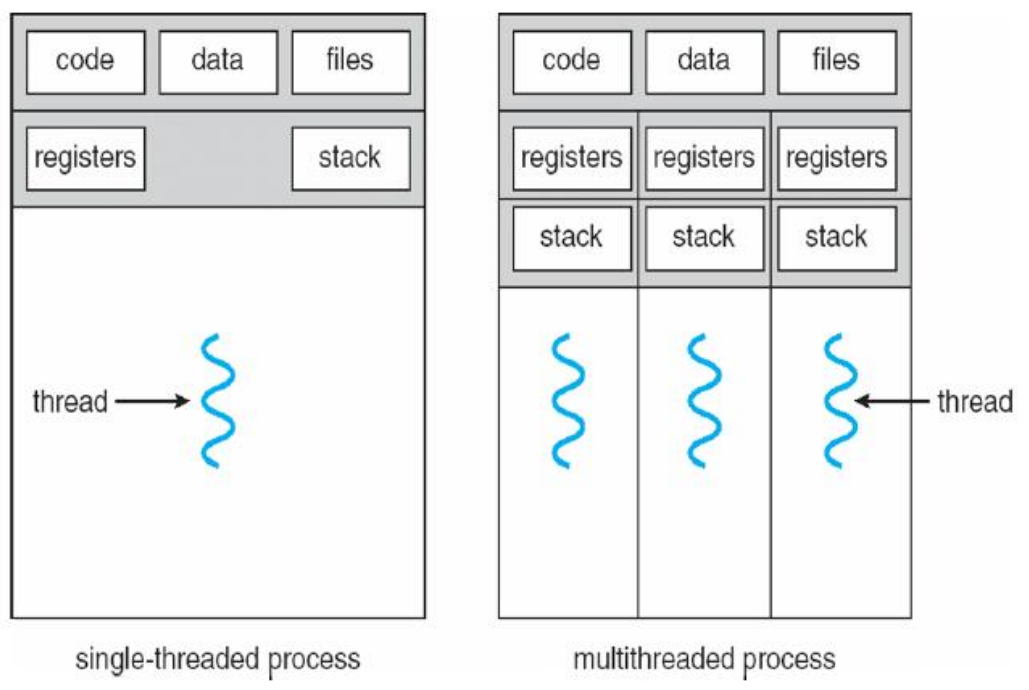
\includegraphics[width=0.33\textwidth]{ProcessesThreads}\end{figure}

\paragraph{Threads --- POSIX}
\begin{items}
  \item \code{PThread}: base object with \\*
    - \emph{identifier} (thread ID, TID) \\*
    - \emph{register set} (including IP and SP) \\*
    - \emph{stack area} to hold execution state
  \item \code{Pthread_create}: create new thread \\*
    - Pass: \emph{pointer} to \code{pthread_t} (will hold TID after successful call) \\*
    - Pass: \emph{attributes}, \emph{start function}, \emph{arguments} \\*
    - Returns: \code{0} on success, error value else
  \item \code{Pthread_exit}: terminate calling thread \\*
    - Pass: exit code (casted to void pointer) \\*
    - Free's resources (e.g. stack)
  \item \code{Pthread_join}: wait for specified thread to exit \\*
    - Pass: \code{ptread_t} to wait for (or \code{-1} for any thread) \\*
    - Pass: pointer to pointer for exit code \\*
    - Returns: \code{0} on success, error value else
  \item \code{Pthread_yield}: release CPU to let another thread run
\end{items}

\paragraph{Threads --- Problems}
\begin{items}
  \item \textbf{Processes vs. Threads}: \\*
    - \emph{Processes}: only share resources explicitly \\*
    - \emph{Threads}: more shared state \( \to \) more can go wrong \\*
  \item \textbf{Challenges}: programmer needs to take care of \\*
    - \emph{activities}: dividing, ordering, balancing \\*
    - \emph{data}: dividing \\*
    - \emph{shared data}: access synchronizing
\end{items}

\paragraph{PCB vs. TCP}
\begin{items}
  \item \textbf{PCB} (\emph{process control block}): information needed to implement processes \\*
    - always known to OS
  \item \textbf{TCB} (\emph{thread control block}): per thread data \\*
    - OS knowledge depends on \emph{thread model}
\end{items}
\begin{figure}[H]\centering\label{PCBTCB}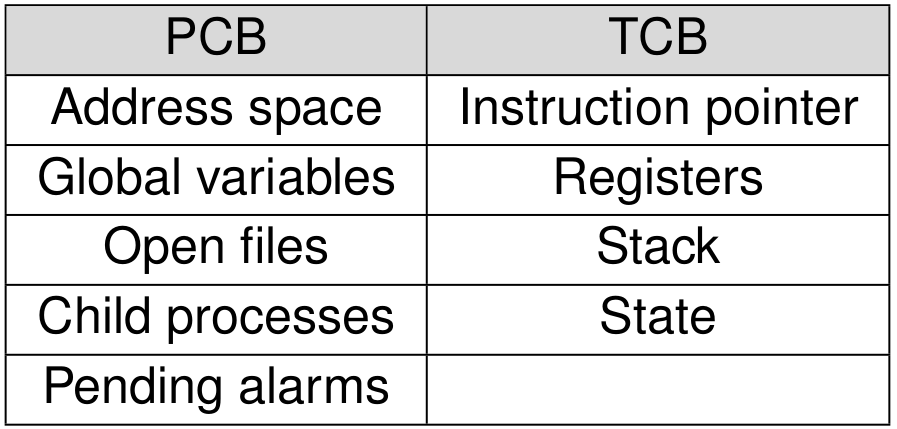
\includegraphics[width=0.2\textwidth]{PCBTCB}\end{figure}

\paragraph{Thread models}
\begin{items}
  \item \textbf{Kernel Thread}: known to OS kernel
  \item \textbf{User Thread}: known to process
  \item \textbf{N:1-Model}: kernel only knows one of possibly multiple threads \\*
    - N:1 user threads = \emph{user level threads} (ULT)
  \item \textbf{1:1-Model}: each user thread maps to one kernel thread \\*
    - 1:1 user threads = \emph{kernel level threads} (KLT)
  \item \textbf{M:N-Model} (hybrid model): flexible mapping of user threads to less kernel threads 
\end{items}

\paragraph{Thread models --- N:1}
\begin{items}
  \item Kernel only manages process \( \to \) multiple threads unknown to kernel 
  \item Threads managed in user-space library (e.g. GNU Portable Threads)
  \item \textbf{Pro}: \\*
    + faster thread management operations (up to 100 times) \\*
    + flexible scheduling policy \\*
    + few system resources \\*
    + usable even if OS doesn't support threads
  \item \textbf{Con}: \\*
    - no parallel execution \\*
    - whole process blocks if one user thread blocks \\*
    - reimplementing OS parts (e.g. scheduler)
  \item \textbf{Stack}: \\*
    - main stack known to OS used by thread library \\*
    - own execution state (= stack) dynamically allocated by user thread library for each thread \\*
    - possibly own stack for each exception handler
  \item \textbf{Heap}: \\*
    - concurrent heap use possible \\*
    - \emph{Attention}: not all heaps are reentrant
  \item \textbf{Data}: divided into BSS, data and read-only data here as well
\end{items}
\begin{figure}[H]\centering\label{ULTAddressSpace}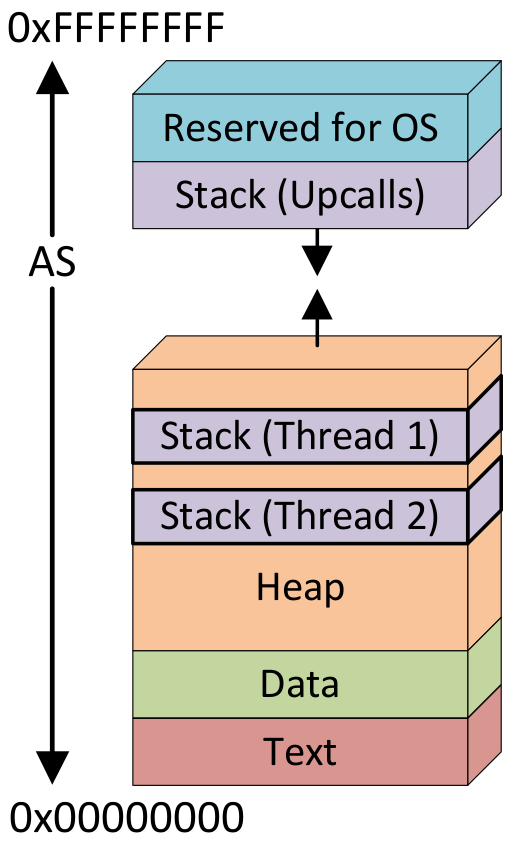
\includegraphics[width=0.15\textwidth]{ULTAddressSpace}\end{figure}

\paragraph{Thread models --- 1:1}
\begin{items}
  \item kernel knows + manages every thread
  \item \textbf{Pros}: \\*
    + real parallelism possible \\*
    + threads block individually
  \item \textbf{Cons}: \\*
    - OS manages every thread in system (TCB, stacks,\dots) \\*
    - Syscalls needed for thread management \\*
    - scheduling fixed in OS
  \item \textbf{Stack}: \\*
    - own execution state (= stack) for every thread \\*
    - possibly own stack for (each) exception handler
  \item \textbf{Heap}: \\*
    - parallel heap use possible \\*
    - \emph{Attention}: not all heaps are thread-safe \\*
    - if thread-safe: not all heap implementations perform well with many threads
  \item \textbf{Data}: divided into BSS, data and read-only data here as well
\end{items}
\begin{figure}[H]\centering\label{KLTAddressSpace}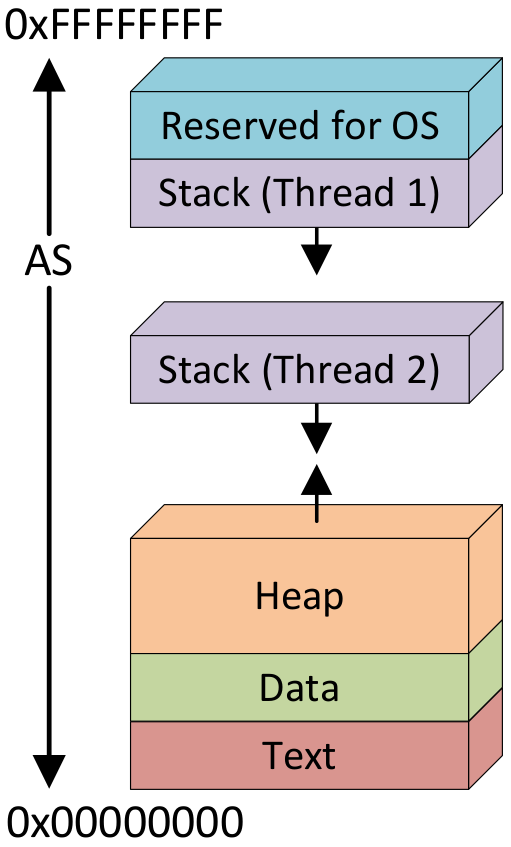
\includegraphics[width=0.15\textwidth]{KLTAddressSpace}\end{figure}

\paragraph{Thread models --- M:N}
\begin{items}
  \item \textbf{Principle}: \( M \) ULTs are maps to (at most) \( N \) KLT \\*
    - \emph{Goal}: pros of ULT and KLT --- non-blocking with quick management \\*
    - create sufficient number of KLTs and flexibly allocate ULTs to them \\*
    - \emph{Idea}: if ULT blocks ULTs can be switched in userspace
  \item \textbf{Pros}: \\*
    + flexible scheduling policy \\*
    + efficient execution
  \item \textbf{Cons}: \\*
    - hard to debug \\*
    - hard to implement (e.g. blocking, number of KLTs,\dots)
  \item \textbf{Implementation --- Up-calls}: \\*
    - kernel notices that thread will block \( \to \) sends signal to process \\*
    - up-call notifies process of thread id and event that happened \\*
    - exception handler of process schedules a different process thread \\*
    - kernel later informs process that blocking event finished via other up-call
\end{items}

\begin{summary}
  \begin{items}
    \item programs often do closely related things at once \\*
      $ - $  mapped to thread abstraction: multiple threads of execution operate in same process
    \item differentiation between process information (PCB) and thread information (TCB)
    \item \textbf{thread models}: \\*
      $ - $ $ N:1 $: threads fully managed in user-space \\*
      $ - $ $ 1:1 $: threads fully managed by kernel \\*
      $ - $ $ M:N $: threads are flexibly managed either in user-space or kernel
    \item multi-threaded programs operate on same data concurrently or even in parallel: \\*
      $ - $ \emph{synchronization}: accessing such data must be synchronized \\*
      $ \to $ makes writing such programs challenging
  \end{items}
\end{summary}